% style notes
% - \,percent not \%

\documentclass[12pt, preprint]{aastex}

% words
\newcommand{\project}[1]{\textsl{#1}}
\newcommand{\thecannon}{\project{The~Cannon}} 
\newcommand{\tc}{\project{The~Cannon}} 
\newcommand{\apogee}{\project{APOGEE}}
\newcommand{\apokasc}{\project{APOKASC}}
\newcommand{\aspcap}{\project{ASPCAP}}
\newcommand{\corot}{\project{Corot}}
\newcommand{\kepler}{\project{Kepler}}
\newcommand{\gaia}{\project{Gaia}}
\newcommand{\gaiaeso}{\project{Gaia--ESO}}
\newcommand{\galah}{\project{GALAH}}
\newcommand{\most}{\project{MOST}}
\newcommand{\code}[1]{\texttt{#1}}
\newcommand{\documentname}{\textsl{Article}}

\newcommand{\teff}{\mbox{$\rm T_{eff}$}}
\newcommand{\kms}{\mbox{$\rm kms^{-1}$}}
\newcommand{\feh}{\mbox{$\rm [Fe/H]$}}
\newcommand{\xfe}{\mbox{$\rm [X/Fe]$}}
\newcommand{\alphafe}{\mbox{$\rm [\alpha/Fe]$}}
\newcommand{\mh}{\mbox{$\rm [M/H]$}}
\newcommand{\logg}{\mbox{$\rm \log g$}}
\newcommand{\noise}{\sigma_{n\lambda}}
\newcommand{\scatter}{s_{\lambda}}
\newcommand{\pix}{\mathrm{pix}}
\newcommand{\rfn}{\mathrm{ref}}
\newcommand{\rgc}{\mbox{$\rm R_{GC}$}}
\newcommand{\vgal}{\mbox{$\rm V_{GAL}$}}

% math
\newcommand{\numax}{$\nu_{\max}$}
\newcommand{\deltanu}{$\Delta\nu$}

\begin{document}

% plotting in /Apogee_ages/makeplot_scatter_test18_step.py 
% and plotelements_on_spectra.py 

\title{Measuring red-giant masses and ages with stellar spectra}
\author{M.~Ness\altaffilmark{1},
David~W.~Hogg\altaffilmark{1,2,3},
H.-W.~Rix\altaffilmark{1},
\textbf{others}}
\altaffiltext{1}{Max-Planck-Institut f\"ur Astronomie, K\"onigstuhl 17, D-69117 Heidelberg, Germany}
\altaffiltext{2}{Center for Cosmology and Particle Physics, Department of Phyics,
             New York University, 4 Washington Pl., room 424, New York, NY, 10003, USA}
\altaffiltext{3}{Center for Data Science, New York University, 726 Broadway, 7th Floor, New York, NY 10003, USA}
% \altaffiltext{4}{NSF Astronomy and Astrophysics Postdoctoral Fellow}
% \altaffiltext{5}{Department of Physics \& Astronomy, Johns Hopkins University, Baltimore, MD, 21218, USA}
\email{ness@mpia.de}

\begin{abstract}%
% Context
With \thecannon, we have demonstrated that it is possible to use a
small training set of stars with noisy spectral data and known
stellar-parameter labels to build a data-driven probabilistic model of
stellar spectra that can be used to infer stellar-parameter labels for
other stars (with differently noisy spectral data).
% Aims
% Method
Here we train this system using stars with known stellar mass labels
obtained from a training set of stars with both
\kepler\ asteroseismological observations (hence the known masses) and
\apogee\ infrared spectral data.
We find that (after training) \thecannon\ can infer stellar
masses---and therefore also stellar ages---for red-giant stars using
infrared spectral data alone.
We produce mass and age labels for all XXX,000 red-giant stars in \apogee\ DR12.
% Results
We demonstrate the validity of the stellar masses and ages by three
methods:
Cross-validation demonstrates that the method obtains (log) mass accuracies of approximately 0.08~dex and (log) age accuracies
of roughly 0.25~dex for typical-quality \apogee\ spectra.
Second, we find that the spectral mass (or age) indicators
discovered by \thecannon\ are associated with elements that can be ``dredged up'',
specifically the CN regions of the spectra and regions that contain C12--C13 [typesetting] blended features. 
Third, we show that the ages of stellar structures in the
Milky Way follow gross expectations, even conditioned on abundances.
All three of these tests show that we can obtain red-giant mass and
age information from stellar spectra; these capabilities open up new
opportunities for Milky Way and stellar astrophysics.
\end{abstract}

\keywords{%
keywords: incomplete (DWH)!
---
methods: data analysis
---
methods: statistical
---
stars: abundances
---
stars: fundamental parameters
---
surveys
---
techniques: spectroscopic
}

\section{Introduction}\label{sec:Intro}

Asteroseismology surveys, such as \most, \corot, and \kepler, have
been extremely successful and productive in bringing us information
about stellar interiors and (therefore) ages.
These missions operate by taking high-cadence, high-precision stellar
photometry, in which stellar oscillation modes are visible in the
Fourier domain.
These missions have operated by taking long stretches of
uninterrupted, uniform, dense imaging data on thousands of individual
stars.
They are expensive missions, but absolutely critical to calibrate
physical stellar interior models and set standards for stellar
parameter estimation, all of which is required for the ultimate
success of the next generation of stellar surveys, particularly
including the \gaia\ Mission.

At the same time, there are many large spectroscopic surveys, such
as \apogee, \galah, and \gaiaeso, underway to measure the properties
of stellar \emph{exteriors}.
These surveys will take high signal-to-noise, high resolution spectra
of hundreds of thousands of stars, revealing detailed surface chemical
abundances.
One question that naturally arises is:
How do we use these two pieces of information (surface spectroscopy
and interior asteroseismology) to jointly infer stellar properties?
Another is:
Is there any way we could learn about stellar interiors from surface
spectroscopy?
After all, at current prices, the marginal cost of taking a spectrum of
a new star is very low relative to the marginal cost of getting its
asteroseismology.
If we can determine the interior properties of stars from surface
spectroscopy alone, even noisily, great opportunities would arise for
studying the stellar populations of the Milky Way and their formation.

\ldots DWH: What are our hypotheses about how mass or age might appear
in a stellar spectrum?  It might appear as dredge-up of evolved
material from the core into the photosphere.  It might appear as
chromospheric emission from a time-dependent magnetic field.  It might
appear as line-shape variations as stellar rotation evolves.  It might
appear as amplitude variations in non-LTE effects as convection scales
are different for stars of different masses.

\ldots DWH: Importantly, age might only appear in the spectra as
certain combinations of surface abundances that are highly covariant
with age.  For example, older stars in the Milky Way tend to be more
alpha-enhanced.  We will consider such age indicators illegitimate;
the purpose of this project is to obtain estimates for ages and masses
\emph{that work even within narrow abundance-selected subsamples}.

\section{Methods and data}

We make use of \tc\ \citep{Ness2015}, which is a data-driven method for
determining stellar parameters and abundances.
\tc\ is a probabilistic model of stellar spectra---meaning that it
produces a likelihood function or a probability density in spectral
space---that is itself a function of stellar parameters and chemical
abundances (which we collectively call ``labels'').
The model is not based on physical models, but is instead learned
from a training set of stars with (assumed) known labels.
This learning is called the ``training step''.
The model is used to label a new star \emph{not} in the training set
by maximizing the likelihood of the label values given the new star's
spectrum.
This labeling is called the ``test step''.
\tc\ differs from other kinds of standard machine-learning methods
(such as random forest or deep neural networks) in that it contains an
explicit likelihood function, at both the training step and the test
step, so it is able to account for heteroskedastic noise and missing
data in the spectra of both the training and test stars.

In detail, the likelihood function we use for \tc\ in this work has a
gaussian form at each measured spectral wavelength, with a mean that
is a quadratic function of the labels, and a variance that consists of
an intrinsic variance added to an observational noise variance (from
photon noise and other sources).
DWH: EQUATIONS HERE.

We have shown in previous work (MKN CITE) that \tc\ does a good job
of modeling stellar spectra and delivering stellar parameters and
chemical abundances for stars with spectra taken by the \apogee\ project.
MKN: DESCRIBE APOGEE BRIEFLY HERE.

One difference between our use of the \apogee\ data and previous work
with the same data is in continuum estimation.
We work with continuum-divided spectra, and the method of continuum
estimation turns out to be important for performance.
MKN: DESCRIBE HOW WE OBTAIN OUR CONTINUUM ESTIMATES HERE.

In this project, we are once again using \apogee\ data, and once again
using \tc.
What's new is that we are adding stellar mass as a stellar parameter
in the label set provided to \tc\ in the training step, and delivered by
\tc\ in the test step.
Stellar mass is a parameter that is not usually considered visible in
spectral data; in the training set we are obtaining these stellar mass
parameters via asteroseismology.

In particular, the training set is taken from the \apokasc\ sample of
stars (MKN CITE).
This sample of stars are in common between the \kepler\ Mission
targets and the \apogee\ targets; they have high-quality infrared
spectra and also asterosesmological measurements.
The \kepler\ Mission (MKN CITE) took continuous, 30-min cadence (or
higher cadence) photometric observations of more than $10^5$ stars,
providing (at least for giant stars) measurements of the
asteroseismological frequencies and frequency splittings that indicate
stellar interior density structure.
The asteroseismological measurements are used---with stellar
models---to infer stellar masses and thus provide labels.

The training set of stars is a subset of 1500 stars from \citet{Martig2015}. These are \apokasc\ stars, with \numax\ and \deltanu\ measurements from \kepler, with corresponding spectra in the H-band across 1.5-1.7 $\micron$ at a resolution of R $\sim$ 22,500, observed as part of the \apogee\ survey. These stars have been selected with no warning or error in the \aspcap\ \code{FLAG} parameter provided by \apogee\ \citep{Ahn2014}, with no rotation flag set and with errors on the delta$\_$nu and nu$\_$max less than 5\,percent. These stars comprise a high signal-to-noise (SNR) sample, with an average SNR $\approx$ 330 $\pm$ 155. 

Five labels are used for training of \tc, the \teff, \logg, \feh, \alphafe\ and Mass. The training labels adopted were the \aspcap-corrected \citep{Meszaros2013} values for the \teff, \feh\ and \alphafe\ and the astroseismic value for \logg, as determined from the measured $\nu_{max}$ . The mass label was determined using the standard seismic scaling relation given in \ref{eqn1} \citep{SilvaAguirre2011,Chaplin2011}.

\begin{equation} \label{eq:mass}
M= \left( \frac{\nu_{\mathrm{max}}}{\nu_{\mathrm{max,\odot}}}\right)^3\  \left( \frac{\Delta \nu}{\Delta \nu_{\odot}}\right)^{-4} \ \left( \frac{T_{\mathrm{eff}}}{T_{\mathrm{eff,\odot}}}\right)^{1.5} \ .
\label{eq1}
\end{equation}
We adopt  $T_{\mathrm{eff,\odot}}=5777$ K, $\nu_{\mathrm{max,\odot}}=3140\ \mu$Hz, $\Delta \nu_{\odot}=135.03\ \mu$Hz. The solar values  $\Delta \nu_{\odot}$ and $\nu_{\mathrm{max,\odot}}$ are the ones used to build the APOKASC catalogue and were obtained by \cite{Hekker2013} with the OCT method.

\section{Validation of mass and age outputs}

For cross validation, we took the 


%(note this improves by 10\,percent from 0.27 to 0.24 if take errors on nu max and delta nu to less than 5 percent. )

%from MM:\\ 
%- error on delta$\_$nu and nu$\_$max lower than 5\,percent (the cut was at 10% before)\\
%- no star in the list of fast rotating stars from Jamie Tayar\\
%- no warning or error in ASPCAPFLAG\\
%- Carbon and Nitrogen abundances $>$-9999\\

\ldots MKN: Some visualization of the trained model and teasers.

\section{Experiments and results}

\subsection{Experiments and results: Interpretation of the residuals}

%%made with run -i /Users/ness/new_laptop/Apogee_ages/makeplot_scatter_test18_step.py
%\begin{figure}[p!]
%\centering
% % \includegraphics[scale=0.31]{./plots/validation.png}
%    \includegraphics[scale=0.51]{./plots/scatter_tgfeh.png}
%  \caption{The first-order coefficients and scatter across the sample regions of the spectra, A and B. Top panel: the baseline spectra representing the first coefficient from the set of reference spectra; middle panel: the next three coefficients ($\theta_1$, $\theta_2$, $\theta_3$),  which correspond to the labels ($\teff, \logg, \feh$); bottom panel: the scatter of the fit with a tenfold expanded vertical scale. The red, blue and green areas in the top panel encompass the wavelength regions with the 5\% highest (absolute value) coefficients for the \feh, \logg\  and \teff\ labels respectively. The \teff\ coefficient has been multiplied by a factor of 1000 simply to show this coefficient on a similar scale to the other coefficients. This indicates where the flux in these spectrum is particularly sensitive to the labels.  Note that the \feh\ label is dominant in the contribution level and from the top panel it is clear that there is significant covariance between the labels and there are only a few regions of \logg\ sensitivity. The filled dots in the baseline spectrum in the top penal indicate the wavelengths at which the dependencies on all labels are weak, which we operatively identify as continuum pixels.}
%\label{fig:validation}
%\end{figure}

% run run -i makeplot_scatter_test18_step/spectra in /Apogee_ages/ o
\begin{figure}[p!]
\centering
 % \includegraphics[scale=0.31]{./plots/validation.png}
    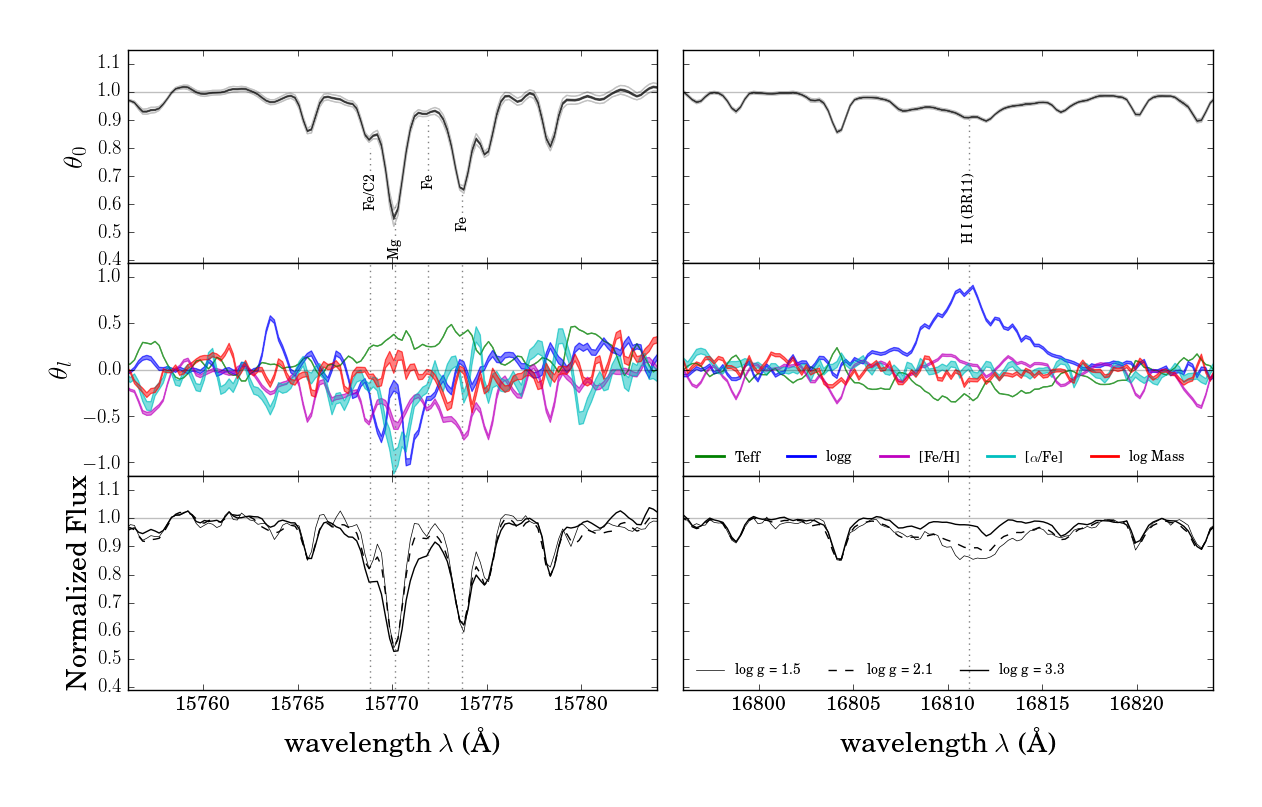
\includegraphics[scale=0.51]{./plots/coeffs_g_3.png}
  \caption{The first order coefficients of the model trained on the \aspcap\ stars showing the two 20 Angstrom wavelength regions where the \logg\ coefficient reaches the highest absolute amplitude. The 0th coefficient (at top) describes the intersect spectrum and relevant spectral absorption features are marked. The lower panel shows all coefficients, each normalised to their highest amplitude, for all \teff, \logg, \feh,\alphafe\ and mass coefficients.}
\label{fig:g}
\end{figure}

Figure \ref{fig:g} shows the two 20 Angstrom regions where the \logg\ coefficient reaches the highest amplitude. The intersect spectra (0th coefficient) is plotted at top and the coefficients for the 5 labels are plotted in the bottom panels.  The left panel includes some of the elements corresponding to the absorption lines. The IR spectral region is highly blended with molecular features and most lines are a blend including CN, C2 and OH features. The maximum amplitude of the \logg\ coefficient does not correspond to the core of the absorption feature of the intersect spectrum but rather the wings. As \logg\ increases, these wings broaden and deepen. Consersely, the panel on the right hand side is the second highest amplitude of the \logg\ coefficient but is positive, The feature this correlates with is the Brackett feature, which becomes shallower and flatter with increasing \logg. 




\subsubsection{Teff residuals}

The strongest \teff residual is at 15720 \AA. 

% run run -i makeplot_scatter_test18/spectra_step in /Apogee_ages/ o
\begin{figure}[p!]
\centering
 % \includegraphics[scale=0.31]{./plots/validation.png}
    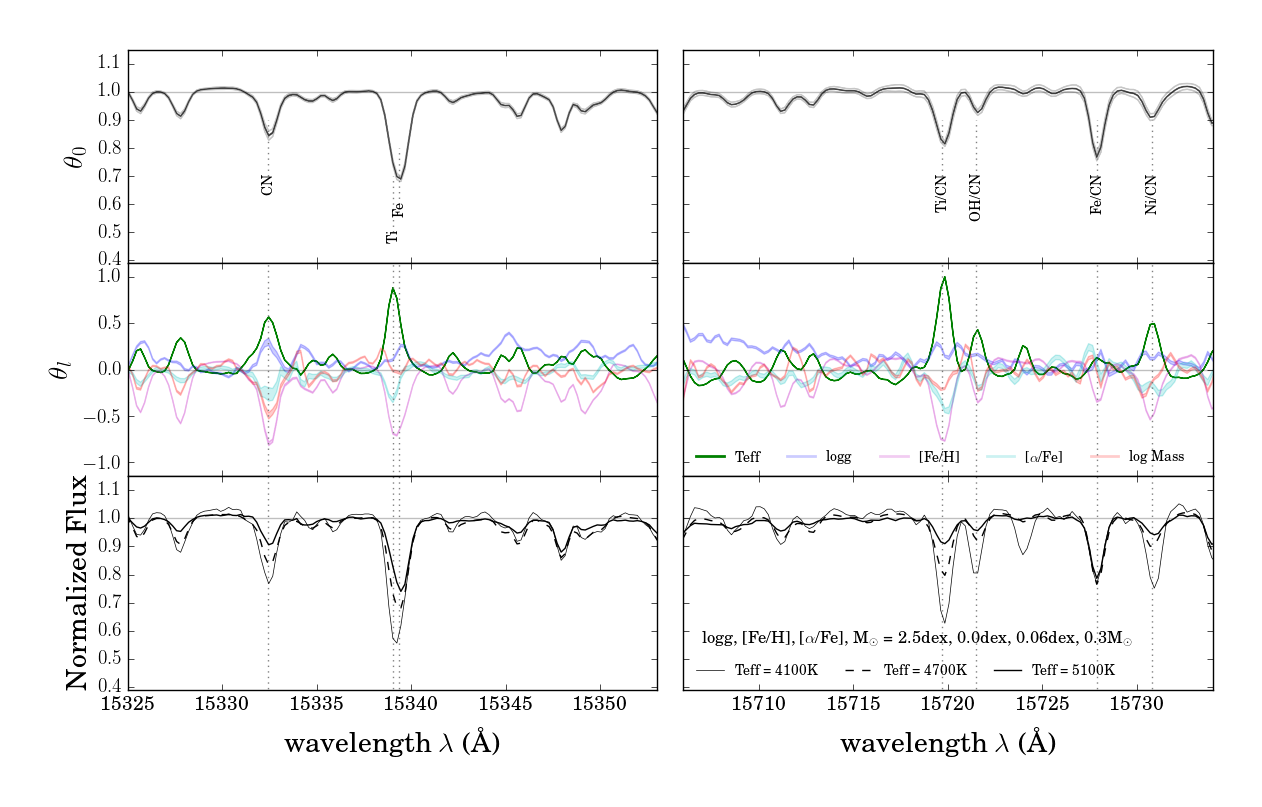
\includegraphics[scale=0.51]{./plots/coeffs_t_3.png}
  \caption{The first order coefficients of the model trained on the \aspcap\ stars showing the two 20 Angstrom wavelength regions where the \teff\ coefficient reaches the highest absolute amplitude. The 0th coefficient (at top) describes the intersect spectrum and relevant spectral absorption features are marked. The lower panel shows all coefficients, each normalised to their highest amplitude, for all \teff, \logg, \feh,\alphafe\ and mass coefficients.}
\label{fig:g}
\end{figure}

This is a Ti I line. \\

% run run -i makeplot_scatter_test18_step_spectra in /Apogee_ages/ o
\begin{figure}[p!]
\centering
 % \includegraphics[scale=0.31]{./plots/validation.png}
    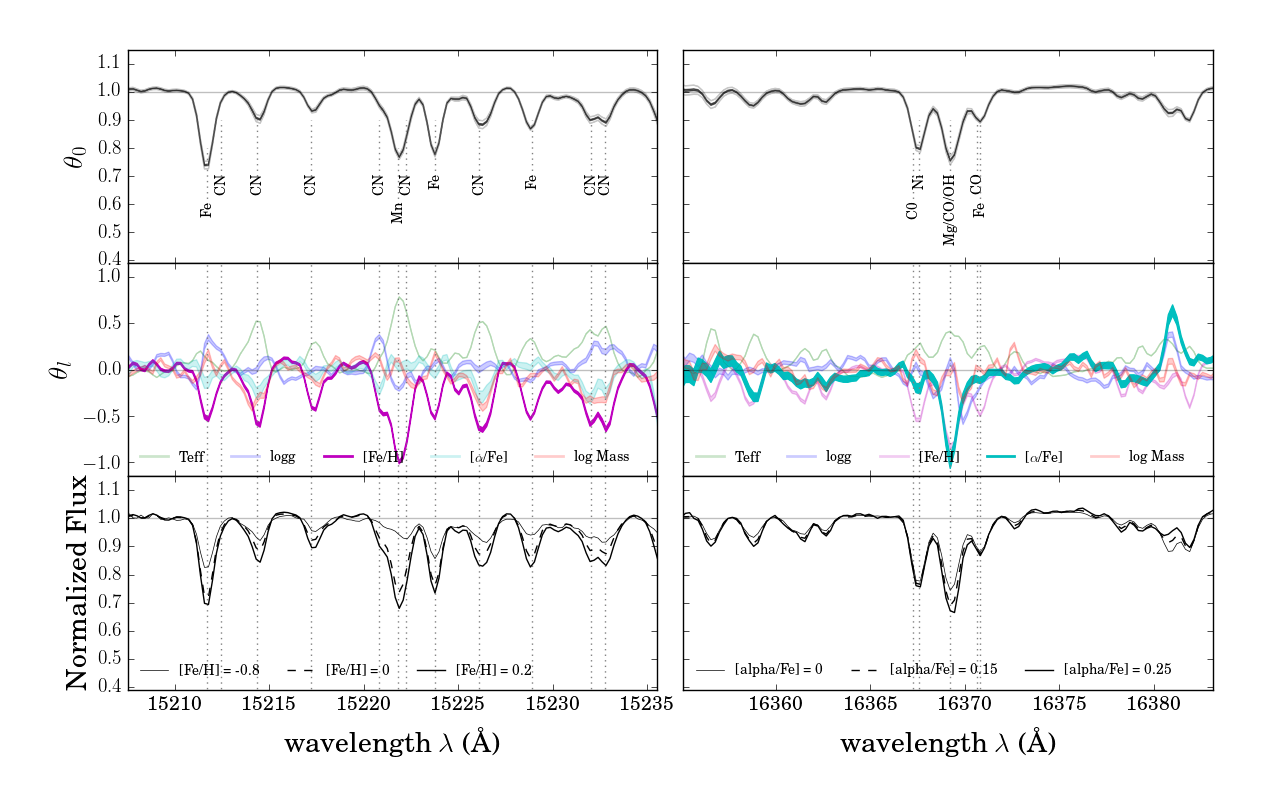
\includegraphics[scale=0.51]{./plots/coeffs_af_3.png}
  \caption{The first order coefficients of the model trained on the \aspcap\ stars showing the two 20 Angstrom wavelength regions where the \teff\ coefficient reaches the highest absolute amplitude. The 0th coefficient (at top) describes the intersect spectrum and relevant spectral absorption features are marked. The lower panel shows all coefficients, each normalised to their highest amplitude, for all \teff, \logg, \feh,\alphafe\ and mass coefficients.}
\label{fig:g}
\end{figure}

\begin{figure}[p!]
\centering
 % \includegraphics[scale=0.31]{./plots/validation.png}
    
\includegraphics[scale=0.51]{./plots/coeffs_m_3.png}
  \caption{The second coefficient is not there if train on linear mass - concerning..}
\label{fig:g}
\end{figure}


%run -i makeredclumpplot.py
\begin{figure}[p!]
\centering
 % \includegraphics[scale=0.31]{./plots/validation.png}
     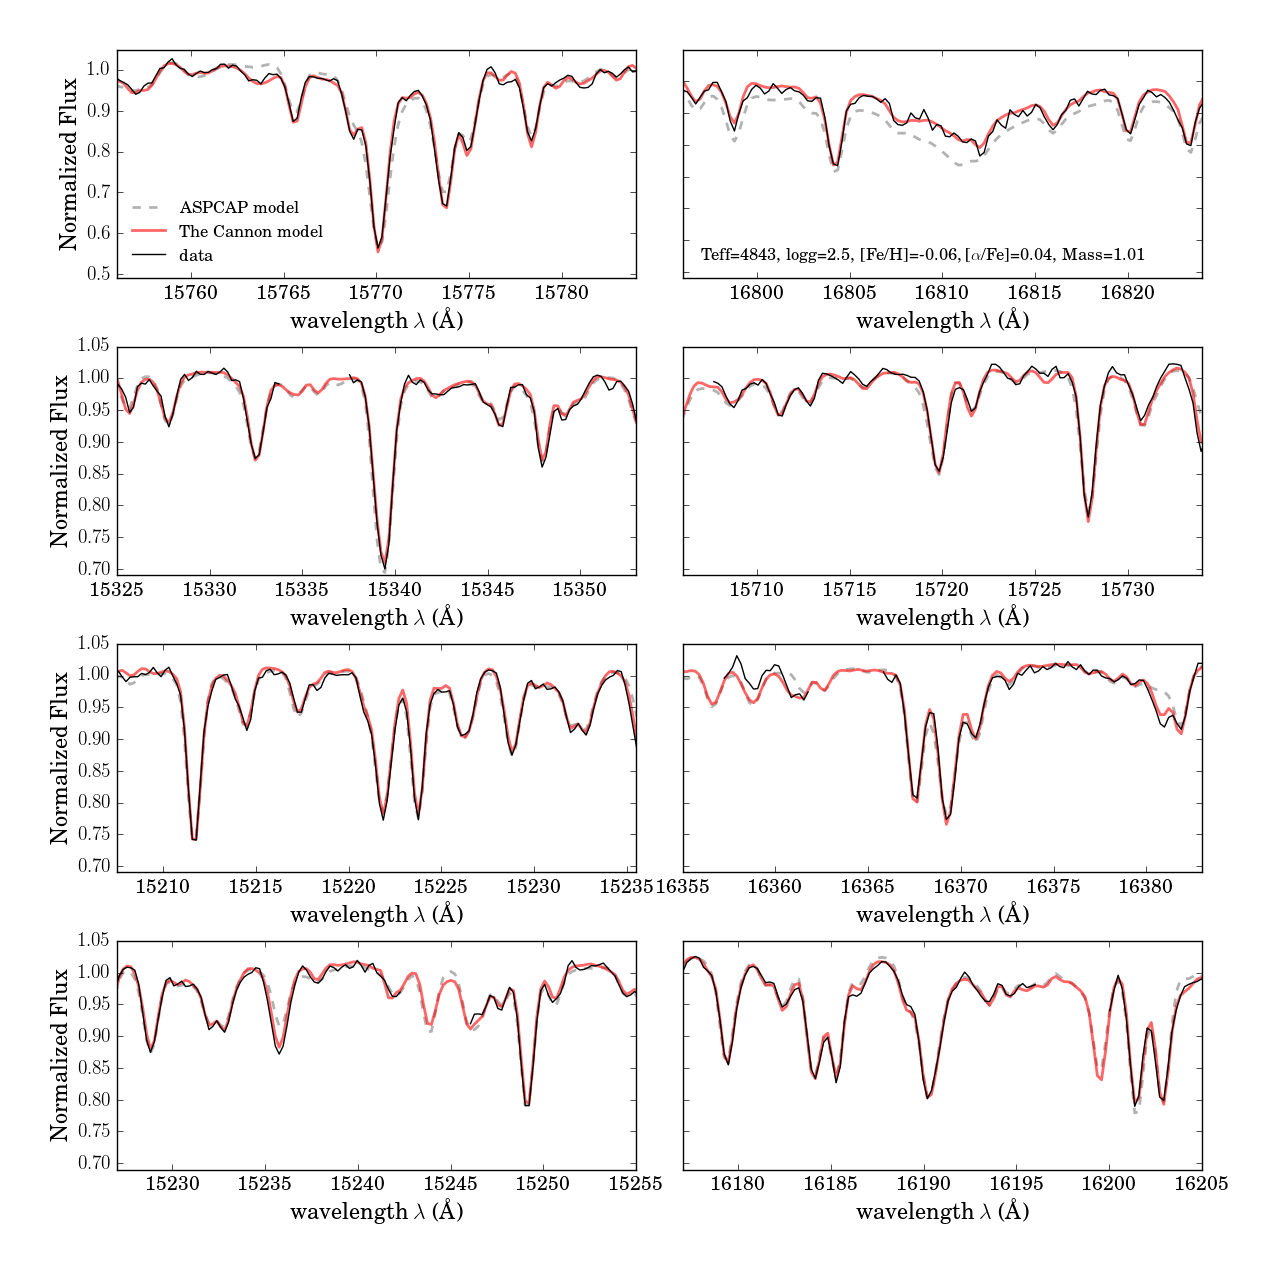
\includegraphics[scale=0.5]{./plots/spectra_fits_7.png}
%    \includegraphics[scale=0.5]{./plots/spectra_fits_7_tg.png}\\
%    \includegraphics[scale=0.5]{./plots/spectra_fits_7_fm.png}
  \caption{fits in regions of logg and teff at top and feh and alphafeh and mass at bottom.}
\label{fig:g}
\end{figure}



\ldots MKN: What is the cross-validation and what are the results?
%plotdiff_5labels_10percent_linear_orig.py trained on 1639 stars if
%run -i plotdiff_5labels_10percent_linear trained on 1500 stars
%/Users/ness/new_laptop/TheCannon/TheCannon/code/ plotdiff_5labels_10percent_contour.py
\begin{figure}[p!]
\centering
 % \includegraphics[scale=0.31]{./plots/validation.png}
 %   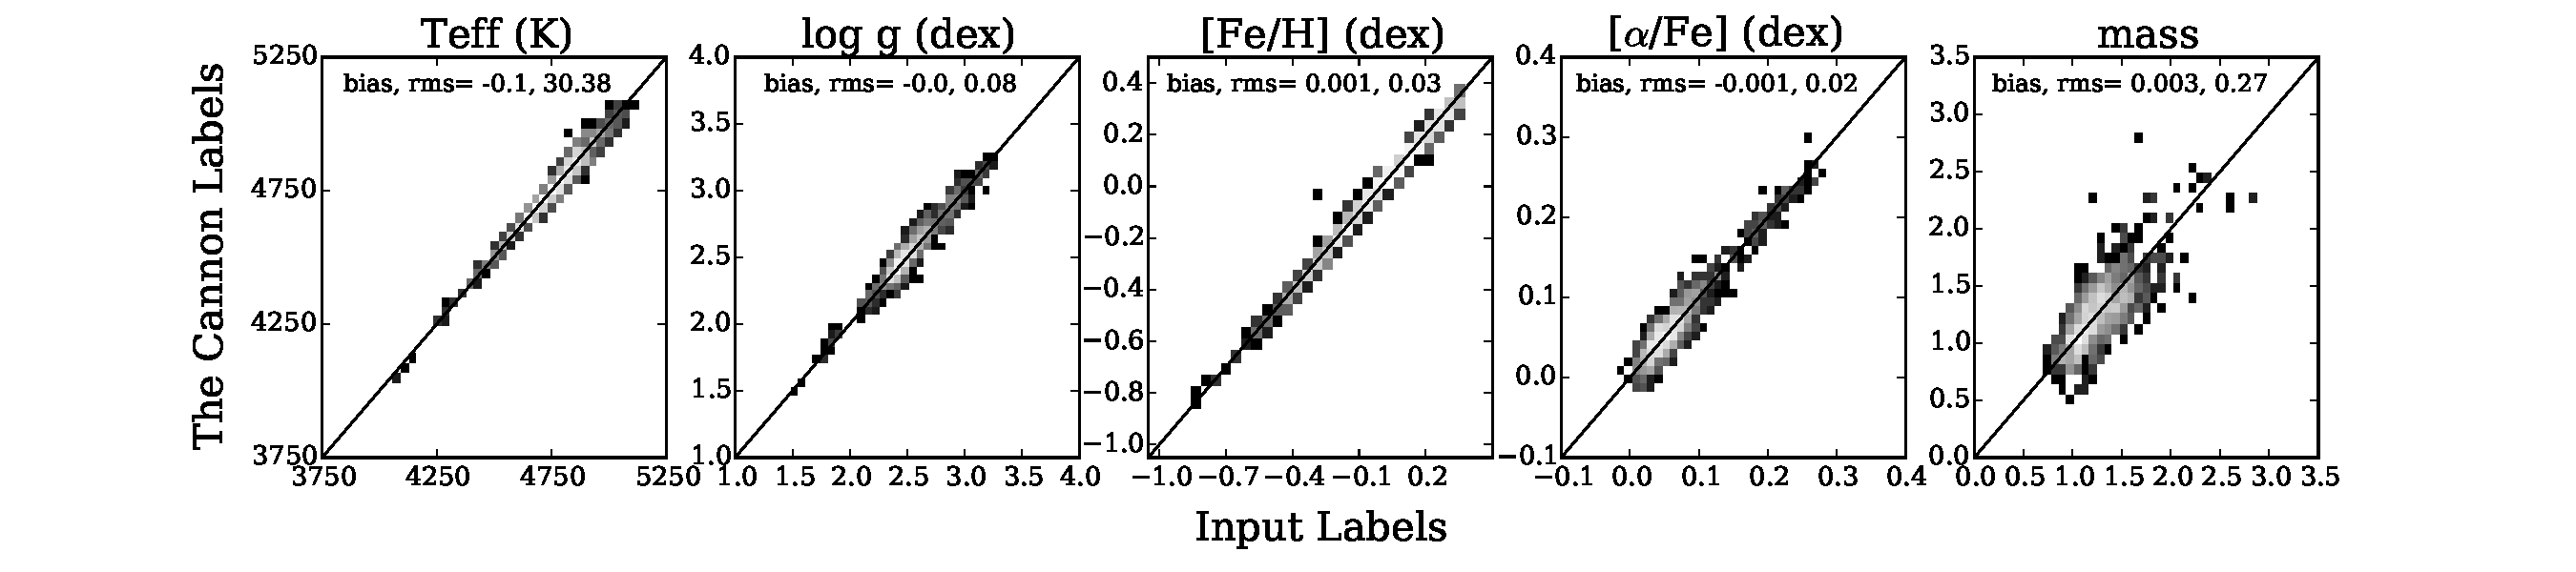
\includegraphics[scale=0.31]{./plots/validation_1500.pdf}
        \includegraphics[scale=0.31]{./plots/validation_1639.pdf}
  \caption{Cross validation of training dataset for the \teff, \logg, \feh, \alphafe\ and mass labels: the results for \tc's labels for training performed on 90\% of the \apokasc\ stars, showing the performance at test time on the 10\% of the stars not included in training, run 10 times.}
\label{fig:validation}
\end{figure}

\begin{figure}[p!]
\centering
 % \includegraphics[scale=0.31]{./plots/validation.png}
 %   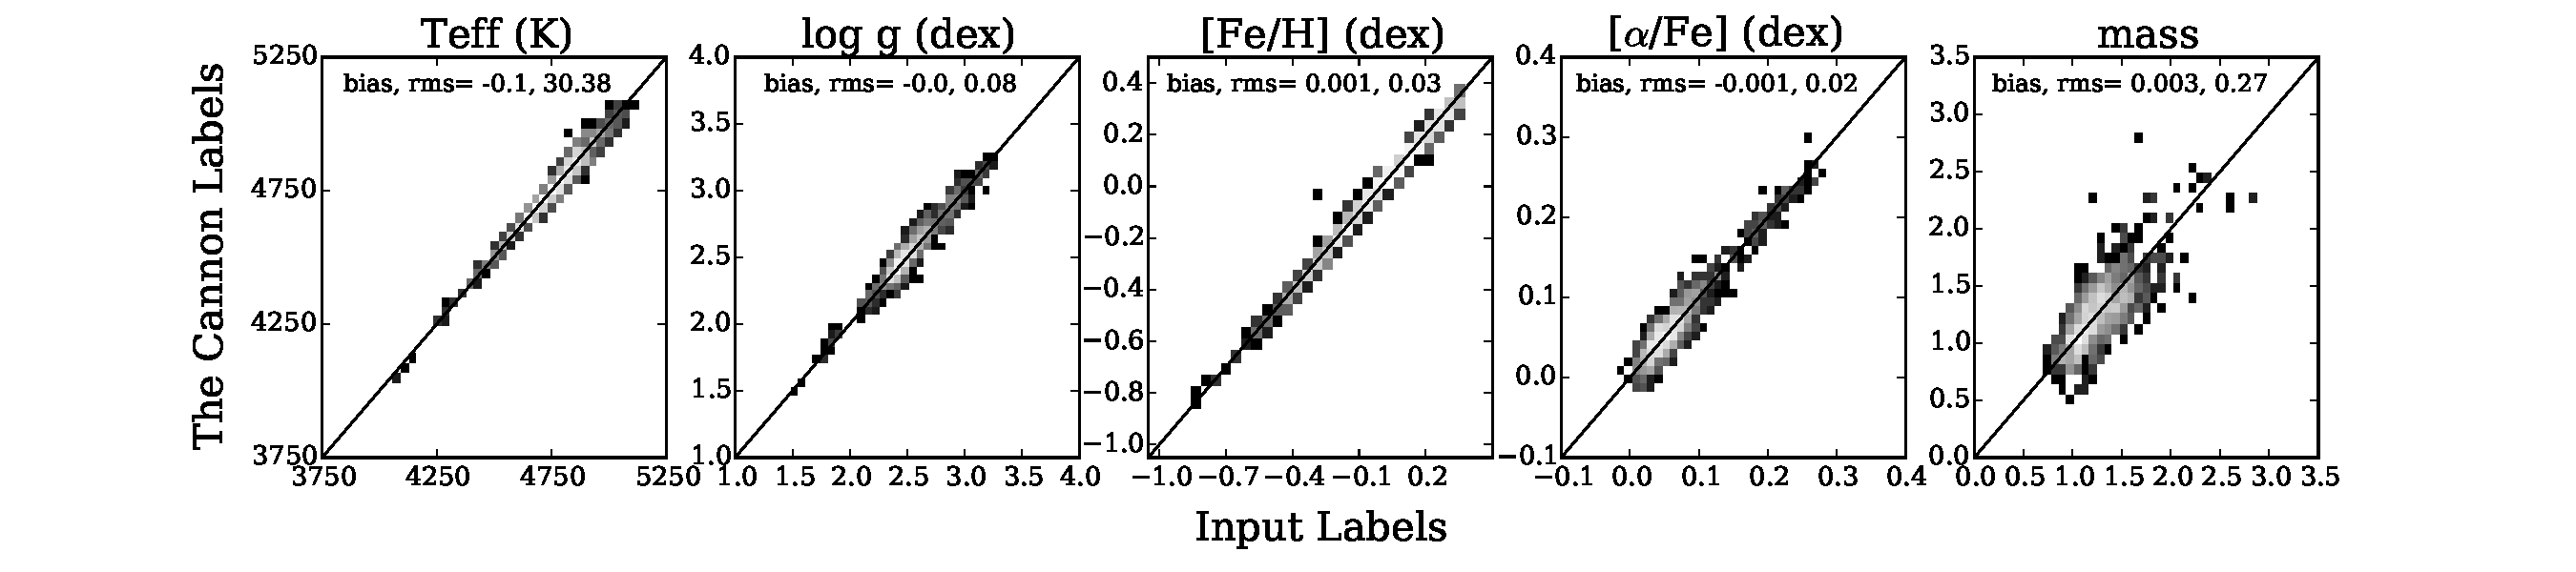
\includegraphics[scale=0.31]{./plots/validation_1500.pdf}
        \includegraphics[scale=0.31]{./plots/validation_1639_ages.pdf}
  \caption{Cross validation of training dataset for the \teff, \logg, \feh, \alphafe\ and age labels (where the mass label has been directly interpolated to mass): the results for \tc's labels for training performed on 90\% of the \apokasc\ stars, showing the performance at test time on the 10\% of the stars not included in training, run 10 times.}
\label{fig:validation}
\end{figure}


\ldots MKN: how do we show that we are simply not reproducing the alpha-\feh\ information:

% made in makealphamap3.py  in Apogee_ages after running plotdiff_5labels2
\begin{figure}[p!]
\centering
 % \includegraphics[scale=0.31]{./plots/validation.png}
    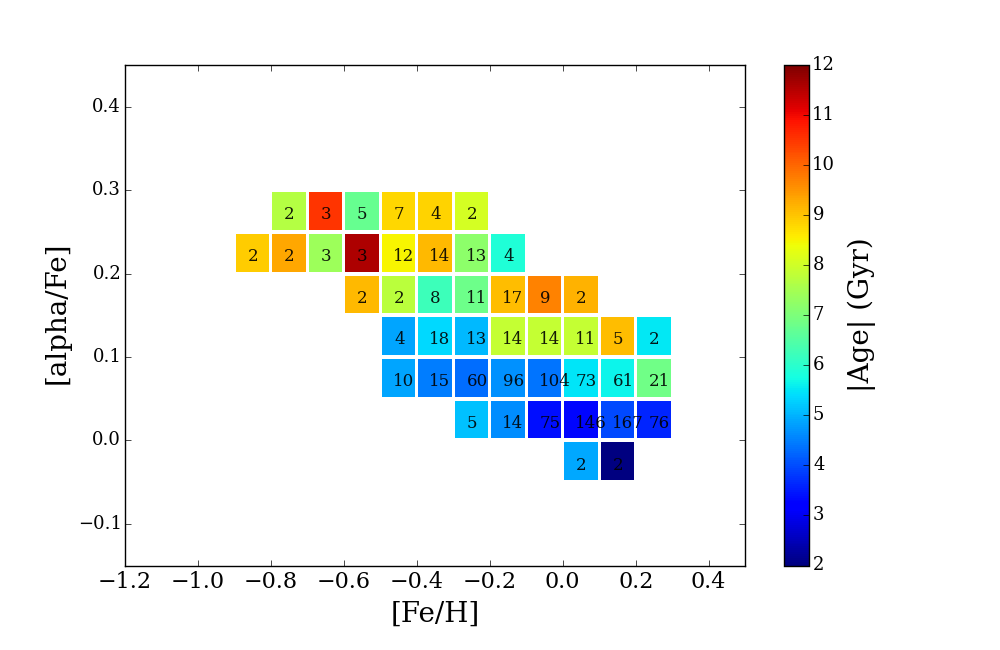
\includegraphics[scale=0.31]{./plots/alpha_feh_bins.png}
    \caption{MKN: Expand to full caption.Bins to test Cannon v. Kepler over  Need to make a less noisy version of this plot from full red clump sample potentially  }
\label{fig:alphabins}
\end{figure}

% made in 
\begin{figure}[p!]
\centering
 % \includegraphics[scale=0.31]{./plots/validation.png}
    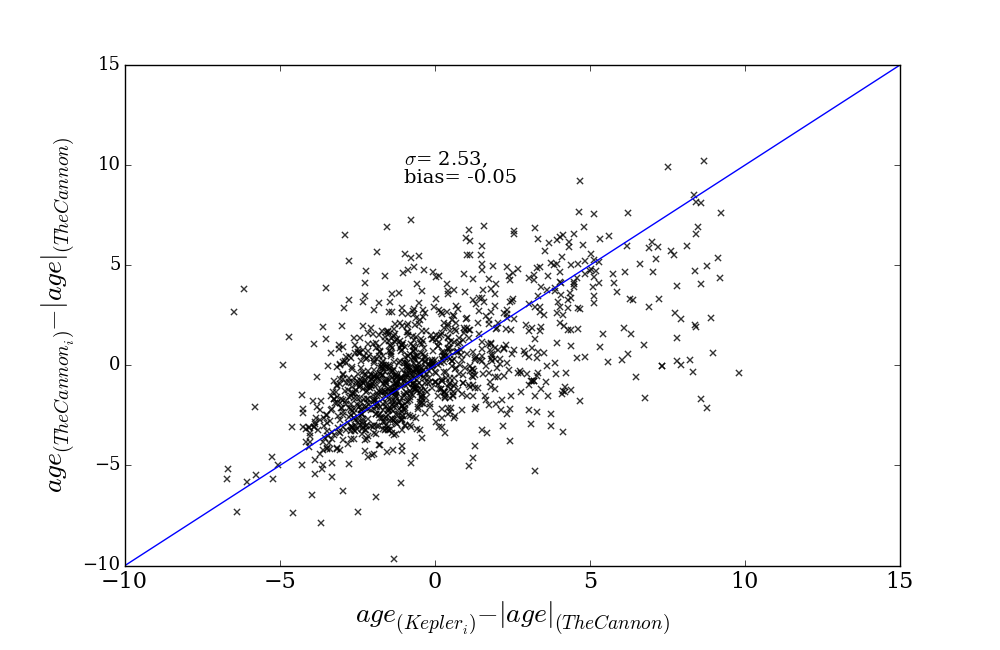
\includegraphics[scale=0.31]{./plots/delta_age_2.png}
    \caption{MKN: Expand to full caption.Bins to test Cannon v. Kepler over  Need to make a less noisy version of this plot from full red clump sample potentially  }
\label{fig:alphabins}
\end{figure}

% made in 
\begin{figure}[p!]
\centering
 % \includegraphics[scale=0.31]{./plots/validation.png}
    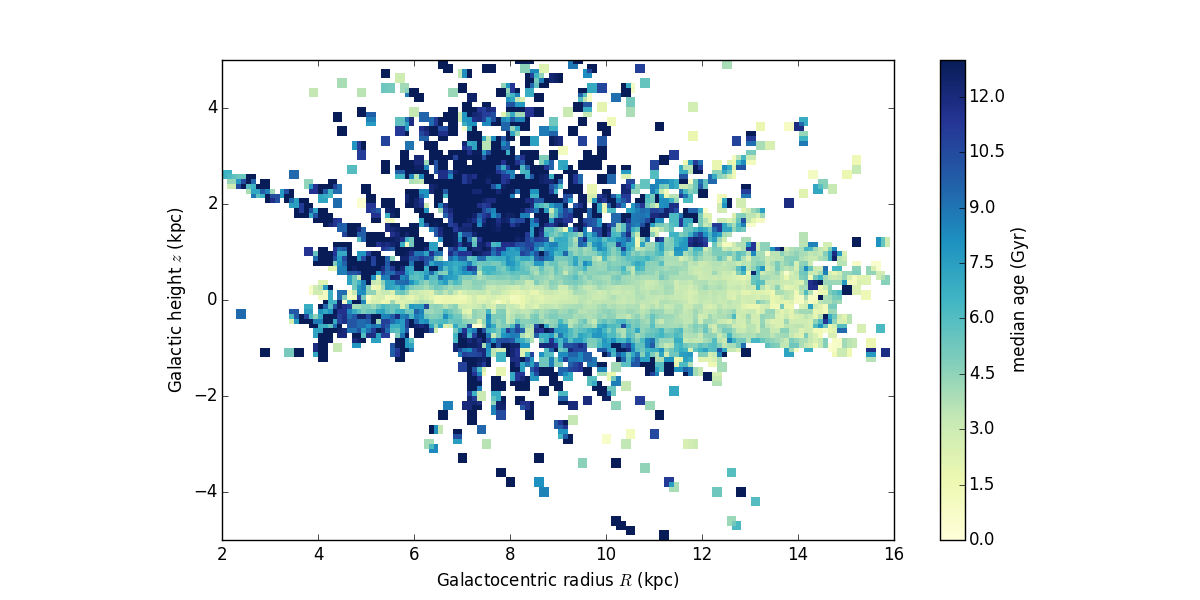
\includegraphics[scale=0.4]{./plots/median_age_abs.png}
    \caption{median age  }
\label{fig:alphabins}
\vspace{-60pt}
\end{figure}

\begin{figure}[p!]
\centering
 % \includegraphics[scale=0.31]{./plots/validation.png}
    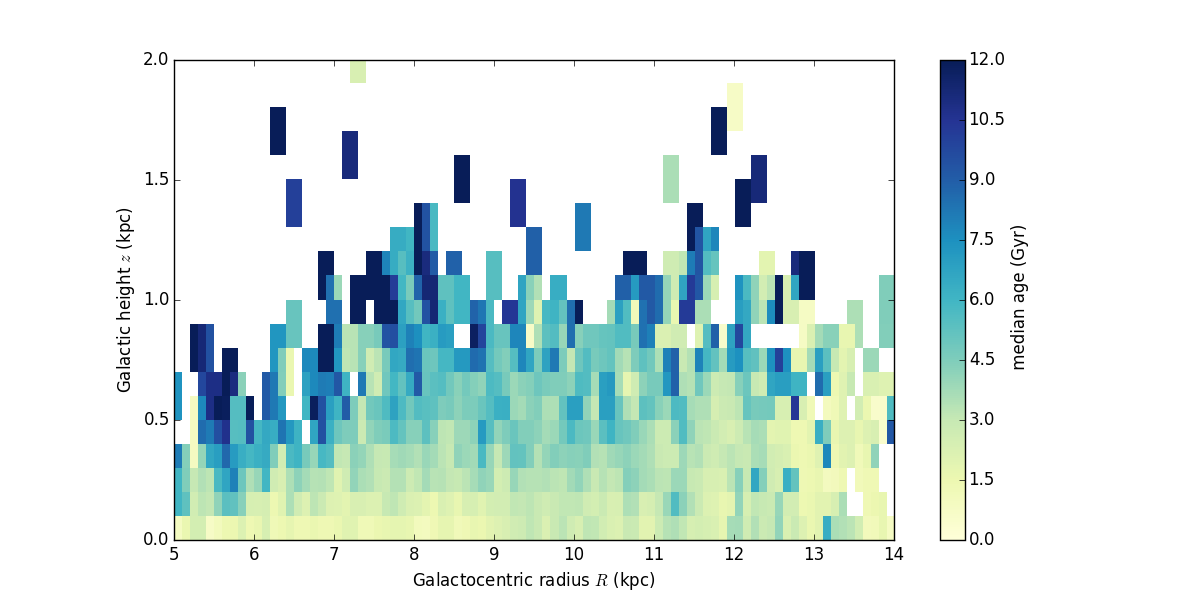
\includegraphics[scale=0.4]{./plots/median_age_low_alpha_abs.png}
    \caption{median age of low alpha sequence = draw where this in in feh alphafeh plane. }
\label{fig:alphabins}
\vspace{-60pt}
\end{figure}

\begin{figure}[p!]
\centering
 % \includegraphics[scale=0.31]{./plots/validation.png}
    \includegraphics[scale=0.4]{./plots/median_age_mono_abs.png}
    \caption{median age of low alpha sequence monoabundance  -  \feh\ is 0 to -0.2. }
\label{fig:alphabins}
\end{figure}

%\begin{figure}[p!]
%\centering
% % \includegraphics[scale=0.31]{./plots/validation.png}
%    \includegraphics[scale=0.3]{./plots/median_age_high_alpha_abs.png}
%    \caption{median age of high alpha sequence = draw where this in in feh alphafeh plane. }
%\label{fig:alphabins}
%\end{figure}

\ldots MKN: What are the spectral signatures of mass and how do they
map on to our hypothesized mass and age indicators?


\ldots MKN: What does the Galaxy look like in terms of age gradients,
in subsamples chosen for chemical homogeneity?

\section{Discussion}

\ldots DWH: Re-cap of what we have achieved and how we know we have
succeeded.

\ldots DWH: Emphasis on the reason that the science result is so
convincing that we really have an age indicator here.

\ldots MKN: What of the hypothesized age indicators are in fact
dominant?

\ldots MKN: How do you obtain our code, data, and results?

\acknowledgments
It is a pleasure to thank
  Foo,
  John Bochanski (Rider),
  Dan Foreman-Mackey (UW), and
  Bar,
for valuable discussions and contributions.
This project made use of
  The NASA Astrophysics Data System,
  and open-source code in the \project{numpy} and \project{scipy} packages.

[Insert SDSS boilerplate here.]

All code and data produced in this project is available HERE and THERE.

\bibliography{tc.bib}

\end{document}
